\chapter{Motor}
\label{cap:p2}

\section{Objectivos}

Com o motor pretende-se uma aplicação que seja capaz de ler um conjunto de pontos especificados em ficheiros XML e .3d e os desenhe numa janela. Além desse objetivo principal foi incluída uma câmara esférica em torno do objeto desenhado e um menu simples que permite alterar o modo de visualização dos pontos.

Nesta secção apresenta-se de que forma o motor foi desenvolvido, começando-se por explicar a leitura dos ficheiros

\section{Leitura Ficheiros}

\subsection{Ficheiro XML}

A estrutura do ficheiro XML contempla apenas dois tipos de elementos:

\begin{itemize}
	\item[\textbf{scene}] - elemento pai
	\item[\textbf{model}] - elemento com 1 atributo \textit{file} cujo valor corresponde ao nome de um ficheiro de pontos
\end{itemize}

A leitura do ficheiro XML é feita pela função:

\begin{Verbatim}
vector<const char *> leXML()
\end{Verbatim}

O valor de retorno da função é um vector de \textit{char *} que contém os nomes dos ficheiros a ser lidos.

O pseudo-codigo da função de leitura do XML pode ser expresso da seguinte forma:

\begin{Verbatim}
vector<const char *> leXML() {
	Abre documento para leitura
	
	if (nao houve erro a abrir o ficheiro) {
		Acede ao primeiro elemento filho de "scene" 
		(que é um elemento "model")
		
		while (houver elementos "model") {
			Vê qual o valor do primeiro atributo 
			do elemento
			
			Coloca o valor do primeiro atributo do
			 elemento no resultado
			 
			Avança para o proximo elemento
		}
	}
	else {
		Informa erro a abrir o ficheiro
	}
	
	Retorna resultado
}
\end{Verbatim}

\subsection{Ficheiros .3d}


Ns ficheiros .3d, cada linha representa um ponto. Em cada linha, existem 3 valores, separados por espaço, correspondentes às coordenadas cartesianas do ponto. É necessário por isso ter uma função que seja capaz de ler os pontos destes ficheiros para que o motor os possa desenhar.

Como referido anteriormente, a função de leitura do XML devolve um vector com os nomes dos ficheiros .3d onde se encontram os pontos a desenhar. Tendo esta lista de ficheiros, o main chama depois a função le3D para cada um dos ficheiros:

\begin{Verbatim}
le3D(const char * ficheiro)
\end{Verbatim}

Esta função recebe como parâmetro o nome de um ficheiro e coloca os pontos do ficheiro num vector de pontos (que é uma variável global). Este vector de pontos será depois o que o motor vai utilizar para desenhar os pontos.

A função le3D() funciona da seguinte forma:

\begin{Verbatim}
void le3D(const char * ficheiro) {
	Abre ficheiro para leitura
	
	while (houver linhas para ler) {
		Coloca numa string o conteudo da linha
		
		Lê os conteudos da linha
		
		Faz um Ponto3D correspondente à linha
		
		Coloca ponto no vector de pontos
	}
	
}
\end{Verbatim}

\section{Desenho dos pontos}

O resultado da leitura do XML e dos ficheiros .3d nele especificados é um conjunto de \textit{Pontos3D} que são armazenados numa variável global. Este conjunto de pontos está implementado sobre a forma de um \textit{vector<Ponto3D>} que é uma variável global ao programa.

A ordem pela qual os pontos aparecem no vector é a ordem pela qual apareceram nos ficheiros, que por sua vez é a ordem pela qual deverão ser desenhados. Nesta situação, desenhar os pontos corresponde simplesmente a percorrer todos os pontos colocados no vector e a pedir ao GLUT para os desenhar. Mostra-se um excerto de código da função renderScene() que corresponde ao desenho dos pontos:

\begin{Verbatim}
glBegin(GL_TRIANGLES);
glColor3f(0.0, 0.0, 1.0);
for (auto it = pontos.begin(); it != pontos.end(); ++it) {
	glVertex3f(it->x, it->y, it->z);
}
glEnd();
\end{Verbatim}

Assume-se que os ficheiros .3d já contêm a ordem correta dos pontos a ser desenhados.

\section{Câmara}

Para se poder ver o objeto desenhado de vários ângulos foi implementada uma câmara colocada sobre uma esfera. Visto que a posição da câmara é um ponto numa esfera, foram usadas coordendas esféricas para gerir o movimento da câmara.

Na secção \ref{p1:cEsfericas} foi apresentada a classe \textit{CoordsEsfericas} que permite torna fácil operações sobre este tipo de coordenadas e respectiva conversão para coordenas cartesianas. Por este motivo, esta classe é ideal para auxiliar a implementação da câmara.

A câmara é representada por uma variável global declarada da seguinte forma:

\begin{Verbatim}
CoordsEsfericas camara;
\end{Verbatim}

À função \textit{gluLookAt()} são passadas as coordenadas cartesianas correspondentes às coordenadas esféricas:

\begin{Verbatim}
gluLookAt(camara.cCartesianas.x,
	camara.cCartesianas.y,
	camara.cCartesianas.z,
	0.0, 0.0, 0.0,
	0.0f, 1.0f, 0.0f);
\end{Verbatim}

É possível ao utilizador mudar a posição da câmara. Os controlos são os seguintes:

\begin{itemize}
	\item[\textbf{Tecla 'W'}] permite ao utilizador ir para cima
	\item[\textbf{Tecla 'S'}] permite ao utilizador ir para baixo
	\item[\textbf{Tecla 'A'}] permite ao utilizador ir para a esquerda
	\item[\textbf{Tecla 'D'}] permite ao utilizador ir para a direita
	\item[\textbf{Tecla 'Q'}] permite ao utilizador afastar-se do objeto
	\item[\textbf{Tecla 'E'}] permite ao utilizador aproximar-se do objeto
\end{itemize}

Estas operações traduzem-se em operações sobre a câmara disponibilizadas pela classe \textit{CoordsEsfericas}:

\begin{Verbatim}
void f_teclas_normais(unsigned char key, int x, int y) {
	switch (tolower(key)) {
		case 'w': camara.paraCima(2 * M_PI / 360.0);  
		break;
		case 's': camara.paraBaixo(2 * M_PI / 360.0); 
		break;
		case 'a': camara.paraEsquerda(2 * M_PI / 360.0);  
		break;
		case 'd': camara.paraDireita(2 * M_PI / 360.0); 
		break;
		case 'e': camara.aproximar(0.5);
		break;
		case 'q': camara.afastar(0.5);
		break;
	}
	glutPostRedisplay();
}
\end{Verbatim}

O efeito de aplicar uma destas operações é a classe \textit{CoordsEsfericas} actualizar os valores das coordenadas esféricas e cartesianas da nova localização da câmara. Assim, quando a função \textit{gluLookAt()} é chamada e acede aos valores de x, y e z da posição da câmara, estes estão atualizados.

\section{Menu}

Para proporcionar alguma flexibilidade na visualização das figuras desenhadas foi incluído um menu que permite ao utilizador alternar entre o modo de visualização de pontos, linhas, ou objeto preenchido:

\begin{figure}[<+htpb+>]
	\centering
	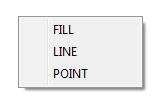
\includegraphics[scale=1.0]{imagens/p1_menuOpcoes.png}
	\caption{Menu de opções de visualização. Acessível com clique no botão direito do rato}
	\label{p1:fig:p1_menuOpcoes}
\end{figure}

O menu foi construído da seguinte forma:

\begin{Verbatim}
glutCreateMenu(menuDrawing);
glutAttachMenu(GLUT_RIGHT_BUTTON);
glutAddMenuEntry("FILL", 0);
glutAddMenuEntry("LINE", 1);
glutAddMenuEntry("POINT", 2);
\end{Verbatim}

O modo de visualização é controlado por uma variável global:

\begin{Verbatim}
GLenum modoPoligonos;
\end{Verbatim}

Quando o utilizador escolhe uma das opções, esta variável é modificada:

\begin{Verbatim}
void menuDrawing(int opt) {
	switch (opt) {
		case 0: modoPoligonos = GL_FILL; break;
		case 1:  modoPoligonos = GL_LINE; break;
		case 2:  modoPoligonos = GL_POINT; break;
	}
	glutPostRedisplay();
}
\end{Verbatim}

O valor da variável é usado na chamada à função \textit{glPolygonMode()} que se encontra na função \textit{renderScene}:

\begin{Verbatim}
glPolygonMode(GL_FRONT_AND_BACK, modoPoligonos);
\end{Verbatim}

\begin{figure}[<+htpb+>]
	\centering
	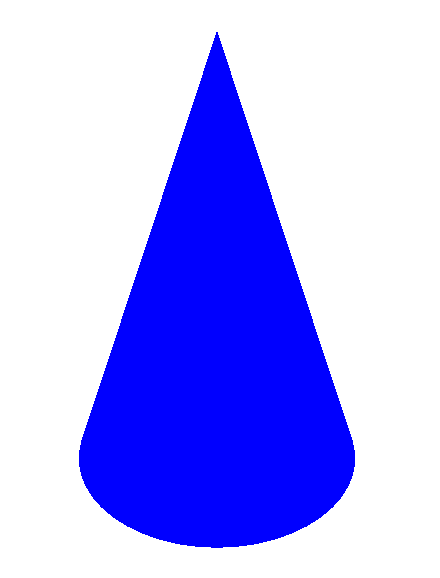
\includegraphics[scale=0.2]{imagens/p1_fill.png}
	\caption{Exemplo de cone construído no modo GL\_FILL}
	\label{p1:fig:p1_fill}
\end{figure}

\begin{figure}[<+htpb+>]
	\centering
	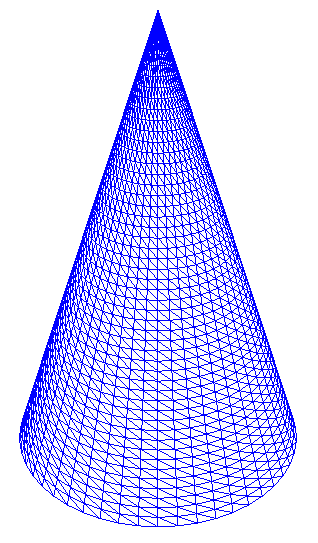
\includegraphics[scale=0.2]{imagens/p1_line.png}
	\caption{Exemplo de cone construído no modo GL\_LINE}
	\label{p1:fig:p1_line}
\end{figure}

\begin{figure}[<+htpb+>]
	\centering
	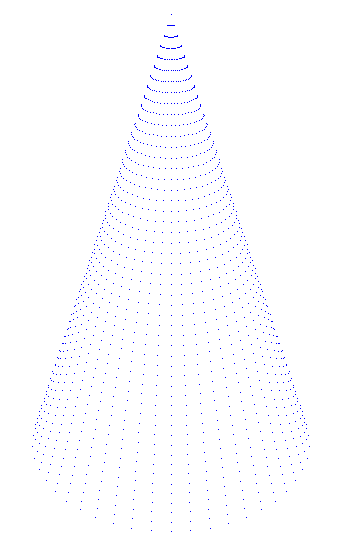
\includegraphics[scale=0.2]{imagens/p1_point.png}
	\caption{Exemplo de cone construído no modo GL\_POINT}
	\label{p1:fig:p1_point}
\end{figure}



